%\documentclass[11pt,a4paper]{article}
%\usepackage{fullpage}
%\usepackage{beamerarticle}
%\documentclass[handout,xcolor=pdftex,dvipsnames,table]{beamer}
\documentclass[hyperref={unicode=true}]{beamer}

%\usepackage{pgfpages} 
%\pgfpagesuselayout{resize}[a4paper,border shrink=5mm,landscape] 

\usepackage[utf8]{inputenc}
\usepackage[russian]{babel}
\usepackage{../clrscode3e} 
%\usepackage[all]{xy}
\usepackage{colortbl}
%\usepackage{xcolor}
\usepackage{pstricks, pst-tree, pst-node}
\usepackage{epsfig}
\usepackage{multicol}
\usepackage{array}
\usepackage{wrapfig}
%\usepackage{listings}
\usepackage{pifont}

\definecolor{orange}{cmyk}{0,0.52,1,0}

%\usepackage{beamerthemesplit}

\AtBeginSection[]
{
  \begin{frame}<beamer>{Раздел}
    \tableofcontents[currentsection]
  \end{frame}
}


\AtBeginSubsection[]
{
  \begin{frame}<beamer>{Раздел}
    \tableofcontents[currentsection,currentsubsection]
  \end{frame}
}


\newtheorem{rtheorem}{Теорема} 
\newtheorem{rdefinition}{Определение} 
\newtheorem{rconsequence}{Следствие} 
%default}
%themesplit}

\title{Арифметическое кодирование}
\subtitle{Дискретный анализ 2012/13}
\author{Андрей Калинин, Татьяна Романова}
\date{11 мая 2013\,г.}
\usetheme{default}
%\usefonttheme{serif}
\usefonttheme[onlymath]{serif}
%\usefonttheme{professionalfonts}
%\usetheme{default} 


\begin{document}

\frame{\titlepage}

\frame
{
  \frametitle{Литература}


  \begin{itemize}
  \item Witten, Moffat, Bell, Managing gigabytes: compressing and
    indexing documents and images.
  \item M.\,J.\,Atallah, Algorithms and Theory of Computation Handbook, 12-4
        Arithmetic Coding
  \end{itemize}
}

\section{Арифметическое кодирование}

\subsection{Основная идея}
\frame[plain]{
  \frametitle{Кодирование $bccb$}
  \begin{center}
  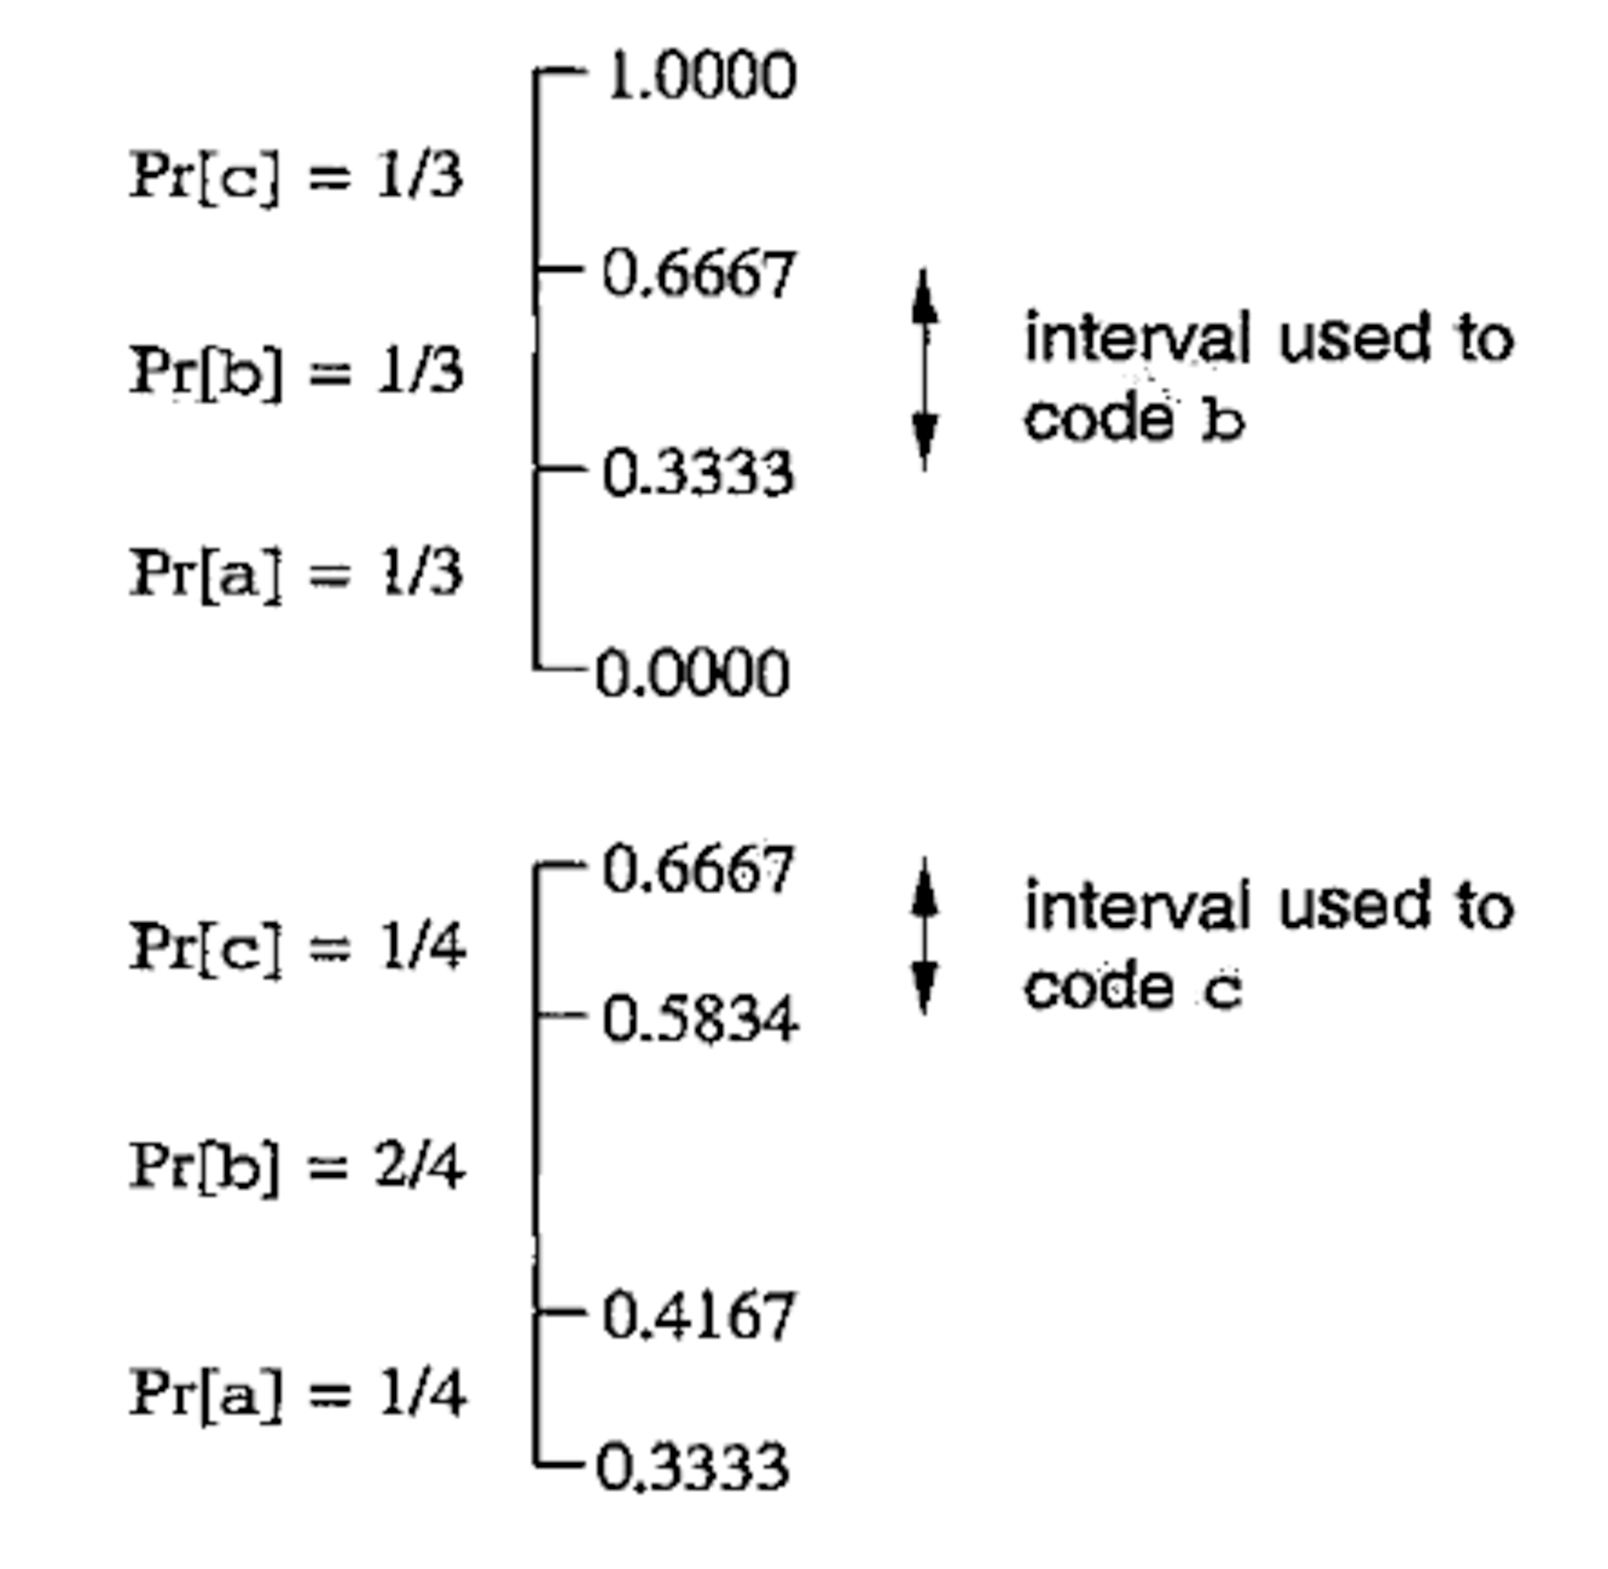
\includegraphics[height=0.8\textheight]{arith-01.eps}
  \end{center}
}
\frame[plain]{
  \frametitle{Кодирование $bccb$}
  \begin{center}
  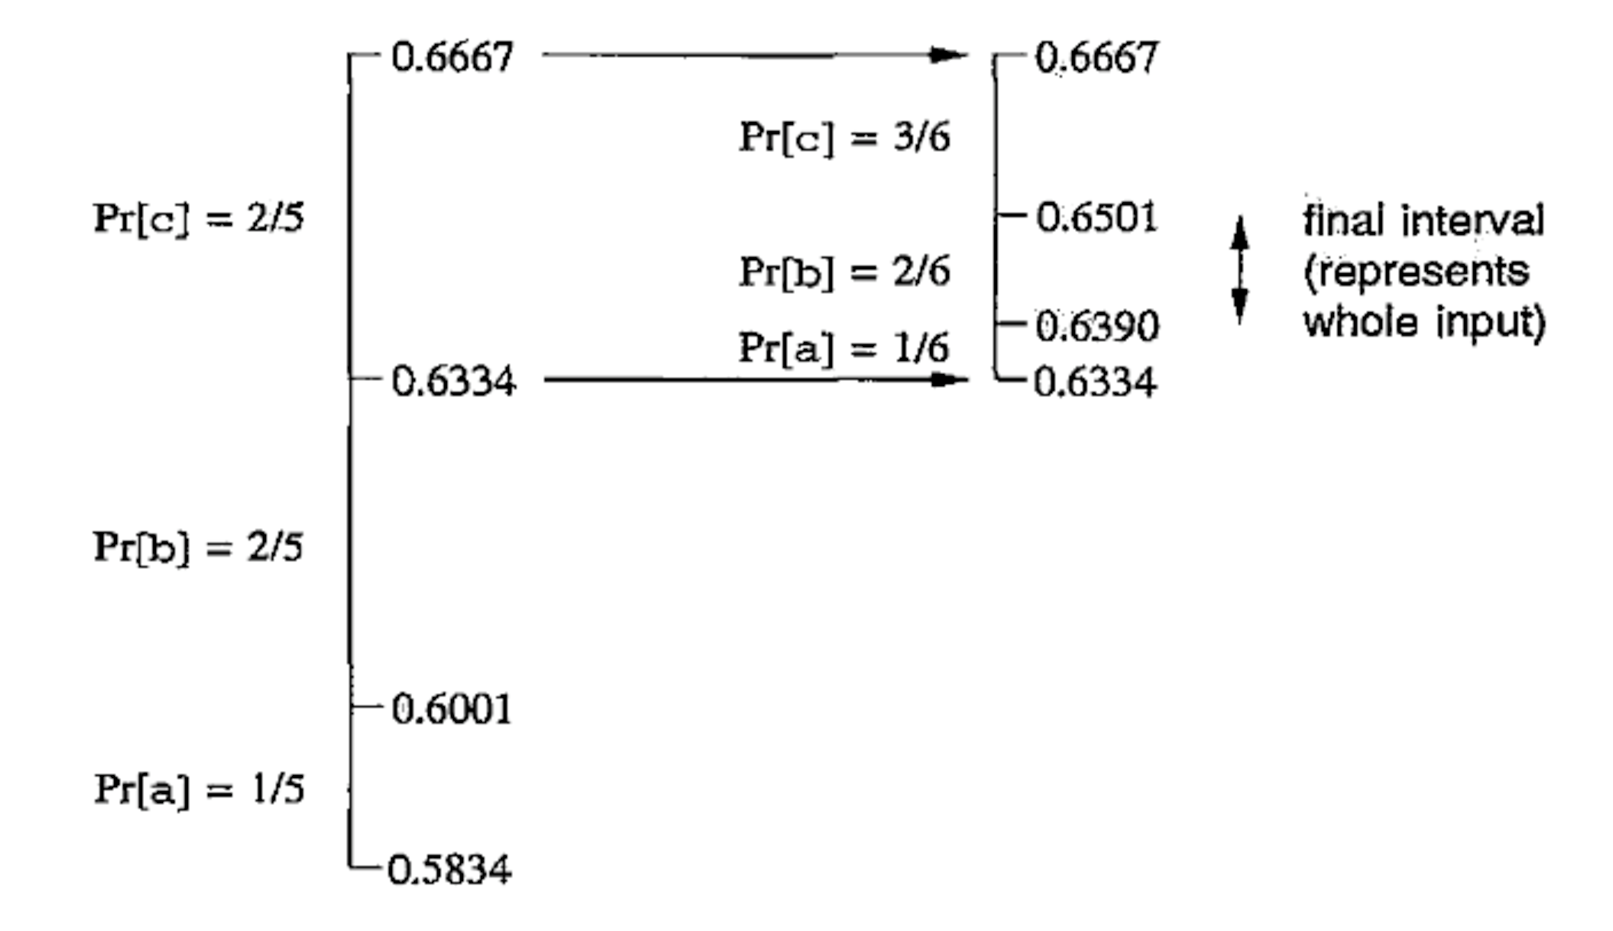
\includegraphics[height=0.8\textheight]{arith-02.eps}
  \end{center}
}
\frame{
  \frametitle{Шаг кодирования}
  \begin{codebox}
    \li $low\_bound \gets \sum_{i=1}^{s-1}P[i]$
    \li $high\_bound \gets \sum_{i=1}^sP[i]$
    \li $range \gets high - low$
    \li $high \gets low + range \times high\_bound$
    \li $low \gets low + range \times low\_bound$
  \end{codebox}
}
\frame{
  \frametitle{Шаг декодирования}
  \begin{enumerate}
  \item Найти $s$ такое, что
    \[
    \sum_{i=1}^{s-1}P[i] \leq \frac{value - low}{high - low} < \sum_{i=1}^sP[i]
    \]
  \item Выполнить все шаги по сужению отрезка, аналогичные шагу кодирования. 
  \item Вернуть символ $s$.
  \end{enumerate}
}

\subsection{Реализация}
\frame {
  \frametitle{Основные моменты}
  \begin{itemize}
     \item Вещественные числа имеют конечную точность. Невозможно закодировать гигабайт текста 64-битным вещественным числом.
     \item Вместо интервала $[0, 1)$ рассмотрим интервал $[0, 2^N - 1)$. Вероятности заменим на количество появлений.
     \item Если левая и правая границы интервала имеют одинаковый префикс, выведем его и расширим интервал. Выведенные биты дадут
           декодеру информацию о текущем интервале.
     \item Если общего префикса нет (середина отерзка между границами), 
            и интервал слишком маленький (меньше, чем кол-во считанных символов), то его тоже нужно расширять,
           не выводя ничего в поток, но и не теряя информацию (нужна дополнительная переменная-счетчик).
  \end{itemize}
}

\frame {
 \frametitle{Кодирование. Реализация. }
  \begin{codebox}
  \Procname{$\proc{AR-Encode-Symbol}(a_i)$}
  \li $l \gets l + ((h - l + 1)*cum\_freq[i])/cum\_freq[0]$
  \li $h \gets l + ((h - l + 1)*cum\_freq[i-1])/cum\_freq[0] - 1$
  \li \Repeat
  \li  \If левый бит $l$ = левому биту $h$
  \li  \Then $\proc{AR-Send-Bit}(leftbit(h))$
  \li        $l \gets 2 * l$
  \li        $h \gets 2 * h + 1$ 
  \li  \Else \If $h - l < cum\_freq[0]$
  \li    \Then $l \gets 2*(l - 2^{N-2})$
  \li          $h \gets 2*(h - 2^{N-2}) + 1$
  \li          $counter = counter + 1$
  \li     \End \End
  \li    \Until левый бит $l$ != левому биту $h$ и $h-l \le cum\_freq[0]$
  \end{codebox}
}

\frame {
 \frametitle{Кодирование. Реализация. }
  \begin{codebox}
  \Procname{$\proc{AR-Send-Bit}(bit)$}
  \li write $bit$
  \li \While $counter > 0$ \Do
  \li    write !$bit$
  \li    $counter = counter - 1$ \End 
  \end{codebox}
}


\frame {
 \frametitle{Кодирование. Пример. }
  Кодируем строчку BBCA. $N = 4, l = 0, h = 15$.\\
  Распределение символов известно заранее: $f(A) = 1, f(B) = 2, f(C) = 1$.\\
  Массив $cum\_freq = [4, 3, 1, 0]$.
  
  1. Считываем символ B (индекс 2 в массиве $cum\_freq$), изменяем границы:
  $$
     l = 0 + (15 - 0 + 1)  * 1 / 4 = 4 = 0100 
  $$
  $$
     h = 0 + (15 - 0 + 1)  * 3 / 4 - 1 = 11 = 1011
  $$
  Общего префикса нет, вывести ничего нельзя, интервал достаточно большой, идем дальше.
  
  2. Считываем символ B:
  $$
     l = 4 + (11 - 4 + 1)  * 1 / 4 = 6 = 0110 
  $$
  $$
     h = 4 + (11 - 4 + 1)  * 3 / 4 - 1 = 0 = 1001
  $$
  Общего префикса нет, вывести ничего нельзя, интервал слишком короткий. 

}

\frame {
 \frametitle{Кодирование. Пример. }
  
  2. Изменяем интервал и увеличиваем $counter$
  $$
     l = (0110 - 0100) << 1 = 0100 = 4 
  $$
  $$
     h = (1001 - 0100) << 1 + 1 = 1011 = 11
  $$
  Общего префикса нет, вывести ничего нельзя, интервал достаточно большой, идем дальше.
  
  3. Считываем символ C:
  $$
     l = 4 + (11 - 4 + 1)  * 0 / 4 = 4 = 0100 
  $$
  $$
     h = 4 + (11 - 4 + 1)  * 1 / 4 - 1 = 5 = 0101
  $$
  Общий префикс 010, после вывода первого бита выводим $counter$ раз его отрицание, а затем все остальное: 0110. 
  Границы после сдвига: 0000 и 1111
}

\frame {
 \frametitle{Кодирование. Пример. }
  
  4. Считываем A
  $$
     l = 0 + 16 * 3 / 4 = 12 = 1100
  $$
  $$
     h = 0 + 16 * 4 / 4 - 1 = 15 = 1111
  $$
  Общий префикс 11 , выводим.
 

  Итого, на выходе: 011011
}

\frame {
 \frametitle{Декодирование. Пример. }
  
  Последовательность: 011011
  
  При декодировании для изменения интервалов делаем те же шаги, что и при кодировании.
  \begin{enumerate}
  \item Из потока считываем первые $N$ бит: $value = 0110 = 6$, видим, что 6 принадлежит интервалу от 4 до 12, следовательно первая буква B.
  \item Изменяем интервал: $l = 4, h = 11$, общих бит нет, $value$ не меняем, оно попадает в интервал от 6 до 19, следовательно вторая буква тоже B.
  \item Изменяем интервал $l = 6, h = 9$, он слишком мал, изменяем границы и $value = 2 * (value - 2^(N - 2))+ bit$.
  \item Новые границы $l = 4, h = 11, value = 0101 = 5$ => следующая буква C.
  \item Изменяем интервал $l = 4, h = 5$ => $value = 1100 = 12$ (биты кончились, дополнили нулями) => следующая буква A.
 \end{enumerate}
  
}






\subsection{Дерево Фенвика}

\frame{
  \frametitle{Основная идея}
  \begin{itemize}
    \item Общие частоты могут быть представлены в виде сумм
      <<подчастот>> для поддиапазонов.
    \item Нужно разделить весь диапазон счётчиков на поддиапазоны,
      которые можно было бы быстрее обходить, чем все счётчики,
      начиная с первого. 
  \end{itemize}
}


\frame[plain]{
\begin{tabular}{ccccccc}
Индекс & Двоичный & Диапазон & Частота & Сумма & Хранится \\
\hline
0 & 0000& 0 & 0 & 0 & 0\\
1 & 0001& 1 & 2 & 2 & 2\\
2 & 0010&1\ldots{}2 & 0 & 2 & 2\\
3 & 0011&3 & 1 & 3 & 1\\
4 & 0100&1\ldots{}4 & 1 & 4 & 4\\
5 & 0101&5 & 1 & 5 & 1 \\
6 & 0110&5\ldots{}6 & 0 & 5 & 1\\
7 & 0111&7 & 4 & 9 & 4\\
8 & 1000&1\ldots{}8 & 4 & 13 & 13\\
9 & 1001&9 & 0 & 13 & 0\\
10 &1010&9\ldots{}10 & 1 & 14 & 1\\
11 &1011& 11 & 0 & 14 & 0\\
12 &1100& 9\ldots{}12 & 1 & 15 & 2\\
13 &1101& 13 & 2 & 17 & 2 \\
14 &1110& 13\ldots{}14 & 3 & 20 & 5\\
15 &1111& 15 & 0 & 20 & 0
\end{tabular}
}


\frame{
  \frametitle{Получение суммарной частоты}
  \begin{codebox}
    \li $S \gets Tree[0]$
    \li \While $i > 0$ \Do
    \li $S \gets S + Tree[i]$
    \li $i \gets i \& (i-1)$ \End
    \li \Return $S$
  \end{codebox}
}

\frame{
  \frametitle{Изменение частоты}
  \begin{codebox}
    \li \Repeat
    \li $Tree[i] \gets Tree[i] + v$
    \li $i \gets i + (i \& -i)$
    \li \Until $i \geq TableSz$
  \end{codebox}
}

\end{document}
